\subsection{Stabilità dei Filtri FIR}
Consideriamo un filtro generico con risposta all'impulso finita, ossia $h(n) = \{h(0),h(1),\dots,h(n)\}$. Sappiamo che per la proprietà di convoluzione
della trasformata Z $Y(z) = H(z)X(z) = \sum_{i = 0}^{M}h(i)z^{-i}X(z)$, allora possiamo riscrivere $H(z)$ come:
\begin{equation*}
    H(z) = \frac{Y(z)}{X(z)} = \frac{\sum_{i = 0}^{M}h(i)z^{-i}\cancel{X(z)}}{\cancel{X(z)}} = \sum_{i = 0}^{M}h(i)z^{-i}
\end{equation*}
Dunque $H(z)$ è un polinomio di grado $M$ e in $\mathbb{C}$ ha esattamente $M$ radici. Riscriviamo allora $H(z)$ in forma fattorizzata:
\begin{align*}
    H(z) &= h(0)(1 - z_1z^{-1})(1 - z_2z^{-1})\dots(1 - z_nz^{-1}) =\\
         &= h(0)\prod_{i = 1}^{M}(1 - z_iz^{-1})
\end{align*}
Avevamo già detto che un filtro digitale è stabile se e solo se tutti i poli sono contenuti nella circonferenza unitaria. Dal momento che 
la funzione di trasferimento di un filtro FIR non ha poli, allora i FIR sono \textbf{intrinsecamente stabili} a prescindere da quale sia la funzione
di trasferimento.

\subsection{Stabilità dei Filtri IIR}
Consideriamo ora un filtro con risposta all'impulso infinita nella sua forma recursiva:
\begin{align*}
    y(n) &= \sum_{i = 1}^{N}a_iy(n - i) + \sum_{i = 0}^{M}b_ix(n - i) =\\
    y(n) - \sum_{i = 1}^{N}a_iy(n - i) &= \sum_{i = 0}^{M}b_ix(n - i)
\end{align*}
Nel \textbf{dominio Z} tutto ciò diventa:
\begin{align*}
    Y(z)\left[ 1 - \sum_{i = 1}^{N}a_iz^{-i}\right] &= X(z)\left[\sum_{i = 0}^{M} b_iz^{-i}\right] \\
    \frac{Y(z)}{X(z)} &= \frac{\sum_{i = 0}^{M} b_iz^{-i}}{1 - \sum_{i = 1}^{N}a_iz^{-i}}\\
    H(z) &=  \frac{\sum_{i = 0}^{M} b_iz^{-i}}{1 - \sum_{i = 1}^{N}a_iz^{-i}}
\end{align*}
Da questa forma della funzione di trasferimento, possiamo notare che ha N poli e M zeri; riscriviamo il tutto come:
\begin{equation}
    H(z) = b_0 \frac{\prod_{i = 1}^{M}(1 - z_iz^{-i})}{\prod_{i = 1}^{(1 - p_iz^{-1})}}
\end{equation}
In questo caso, un filtro IIR è stabile se e solo se $\forall i |p_i| < 1$


\subsection{Sintesi di Filtri Digitali}
In questo campo esistono molte tecniche diverse di sintesi di filtri; una delle più famose e importanti consiste nel \textit{tradurre} l'equazione
alle differenze del sistema nel filtro HW vero e proprio. Per la realizzazione di un filtro digitale sono necessari alcuni componenti base:
\paragraph{Convertitore Analogico-Digitale}
Come abbiamo visto, per poter trattare un segnale digitale dobbiamo prima \textbf{campionarlo} e \textbf{quantizzarlo}. Questa funzione viene svolta 
da un elemento ADC che possiamo rappresentare cosi:
\begin{center}
    \begin{tikzpicture}[node distance=2cm, auto]

        % ADC shape: rectangle with triangular left side
        \draw[thick] (0, 0.5) -- (-1, 0) -- (0, -0.5) -- (2, -0.5) -- (2, 0.5) -- (0, 0.5) -- cycle;
        \node at (0.75, 0) {\textbf{ADC}};
        % Input signal (arrow pointing to the triangle)
        \node[left] at (-1.5, 0) {$s(t)$};
        \draw[->] (-1.5, 0) -- (-1, 0);
        
        % Clock signal (arrow pointing down to the ADC)
        \node[above] at (1, 1) {Clock $f_s$};
        \draw[->] (1, 1) -- (1, 0.5);
        
        % Output (N-bit quantization)
        \node[right] at (3, 0) {$s(n)$ in $N$ bit};
        \draw[->, draw, strike out] (2, 0) -- (3, 0);
        
        \end{tikzpicture}
\end{center}

\paragraph{Ritardatore}
Il ritardatore è un elemento che ritarda di 1 clock un campione. VIene realizzato come un vero e proprio registro, ossia
una batteria di flip-flop che al clock fanno passare in uscita i bit in entrata. Noi lo rappresentiamo come:
\begin{center}
    \begin{tikzpicture}[node distance=2cm, auto]

        % Rectangle with z^{-1} inside
        \node[draw, rectangle, minimum width=1cm, minimum height=1cm] (block) {\( z^{-1} \)};
        
        % Input x(n)
        \node[left of=block, node distance=3cm] (input) {\( x(n) \)};
        \draw[->, thick] (input) -- (block.west);
        
        % Output x(n-1)
        \node[right of=block, node distance=3cm] (output) {\( x(n-1) \)};
        \draw[->, thick] (block.east) -- (output);
        
        % Clock signal
        \node[above of=block, node distance=1.5cm] (clock) {Clock \( f_s \)};
        \draw[->, thick] (clock) -- (block.north);
        
        \end{tikzpicture}
\end{center}
Un ritardatore viene anche chiamato $z^{-1}$ poichè nel dominio Z:
\begin{equation}
    x(n - 1) \zTransform X(z)z^{-1}
\end{equation}

\paragraph{Moltiplicazione}
Un moltiplicatore a $n$ bit moltiplica gli n bit del segnale in ingresso con una costante e in uscita ha n bit. Viene rappresentato così:
\begin{center}
    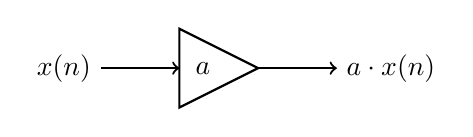
\begin{tikzpicture}[node distance=2cm, auto]

        % Triangle pointing right
        \draw[thick] (1,0) -- (0,0.5) -- (0,-0.5) -- cycle;
        
        % Label inside the triangle
        \node at (0.3, 0) {\( a \)};
        
        % Input x(n)
        \node[left] at (-1,0) {\( x(n) \)};
        \draw[->, thick] (-1,0) -- (0,0);
        
        % Output a*x(n)
        \node[right] at (2,0) {\( a \cdot x(n) \)};
        \draw[->, thick] (1,0) -- (2,0);
        
        \end{tikzpicture}
\end{center}

\paragraph{Sommatore}
Un sommatore somma i segnali in ingresso bit a bit, come un sommatore presente nelle ALU della CPU:
\begin{center}
    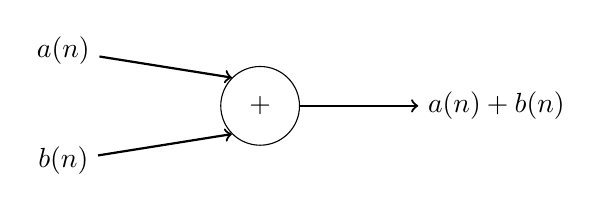
\begin{tikzpicture}[node distance=2cm, auto]

        % Circle with +
        \node[draw, circle, minimum size=1cm] (sum) {\( + \)};
        
        % Input a(n)
        \node[left of=sum, yshift=0.7cm, node distance=2.5cm] (inputA) {\( a(n) \)};
        \draw[->, thick] (inputA) -- (sum.135);
        
        % Input b(n)
        \node[left of=sum, yshift=-0.7cm, node distance=2.5cm] (inputB) {\( b(n) \)};
        \draw[->, thick] (inputB) -- (sum.225);
        
        % Output a(n) + b(n)
        \node[right of=sum, node distance=3cm] (output) {\( a(n) + b(n) \)};
        \draw[->, thick] (sum) -- (output);
        
        \end{tikzpicture}
\end{center}

\paragraph{Esempi di filtri digitali} Alcuni esempi di filtri digitali studiati sono i filtri a pettine (una sorta di filtro passa-basso reale) e i filtri notch (un filtro arresta-banda reale).

\subsection{Filtri a Pettine}
I filtri a pettine sono una famiglia di filtri che hanno la seguente funzione di trasferimento:
\begin{equation}
    H(z) = \frac{1 - z^{-M}}{1 - z^{-1}}
\end{equation}
Dove $M$ è l'\textbf{ordine del filtro}. Scriviamo l'equazione recursiva:
\begin{align*}
    H(z) &= \frac{Y(z)}{X(z)} = \frac{1}{M} \left(\frac{1 - z^{-M}}{1 - z^{-1}}\right)\\
         Y(z) &= \frac{1}{M}X(z)\left(\frac{1 - z^{-M}}{1 - z^{-1}}\right) =\\
         Y(z) &= \frac{1}{M}\left(X(z) - X(z)z^{-M} + Y(z)z^{-1}\right) 
\end{align*}
Antritrasformando otteniamo:
\begin{equation}
    y(n) = \frac{1}{M}\left(y(n-1) + x(n) - x(n - M)\right)
\end{equation}
Dove la $\frac{1}{M} $serve per normalizzare. Possiamo apprendere dalla funzione di trasferimento ha M zeri e 1 polo.
Applicando un polo laddove c'è uno zero, possiamo annullare l'effetto dello zero e non annullare la frequenza in 0.
L'utilità di questo filtro è che è un modesto filtro passa-basso, perchè ha la seguente risposta in frequenza:\\
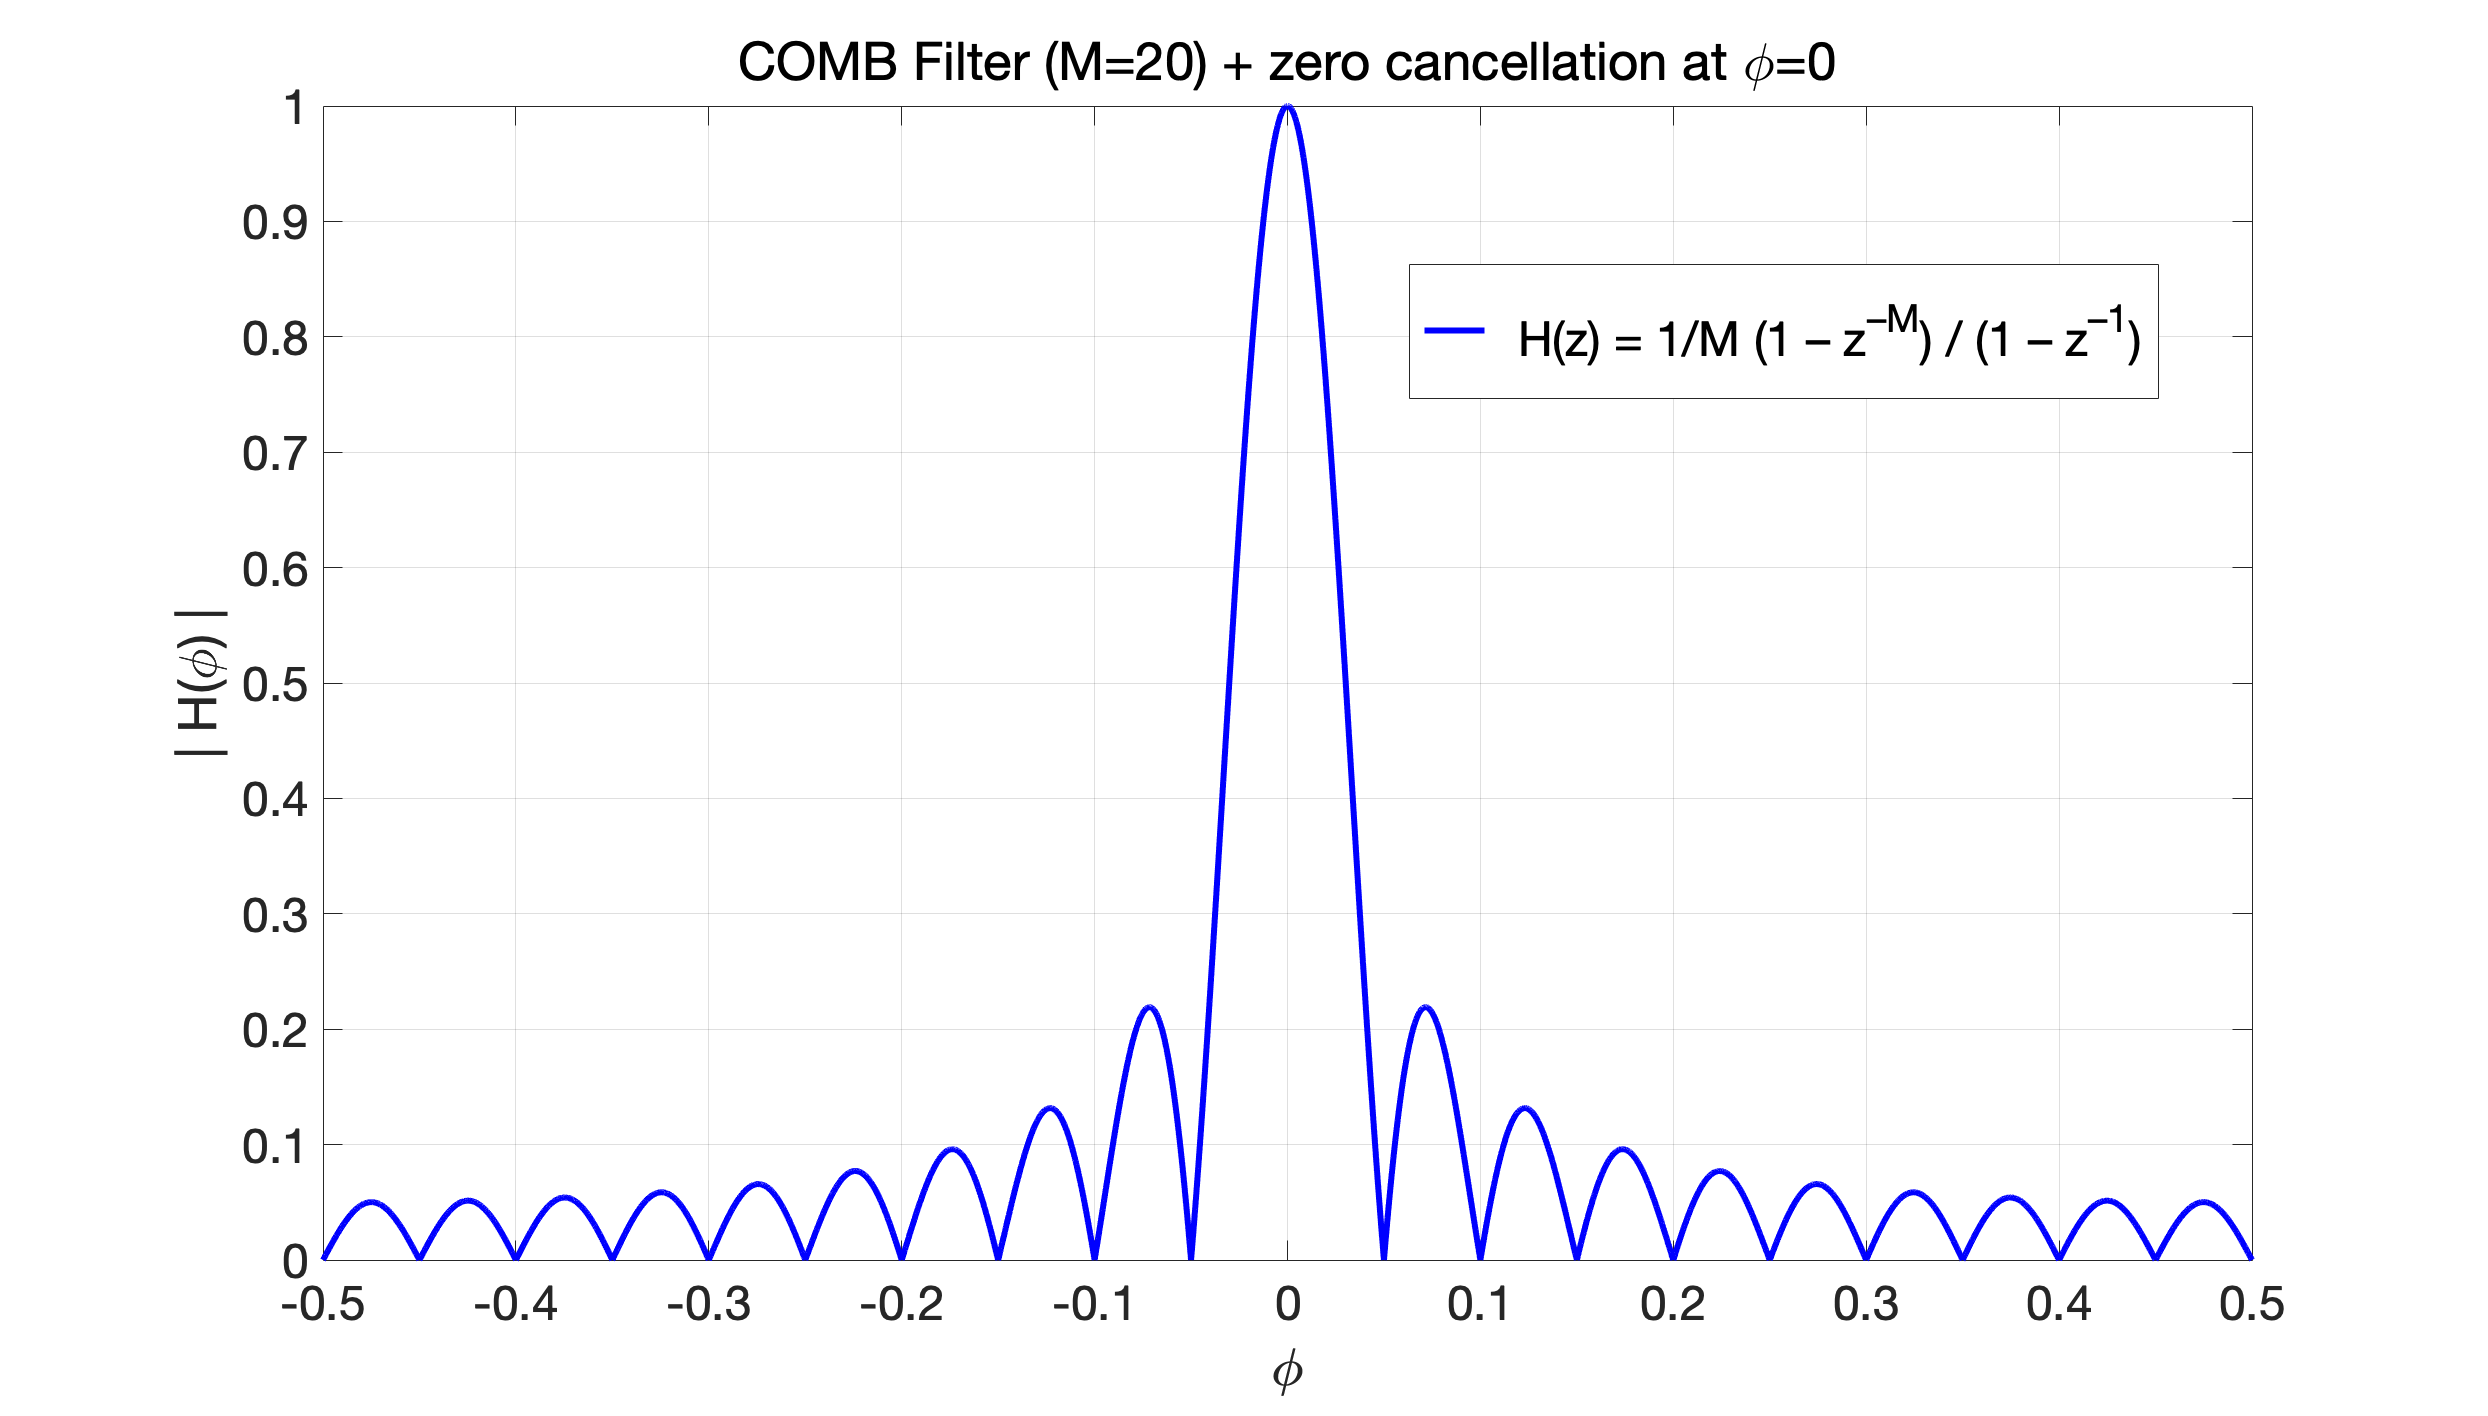
\includegraphics[width=15cm]{src/Comb20Filter.png}
Il lobo centrale fa passare tutto, mentre i lobi laterali attenuano sempre di più. Chiaramente le prestazioni
di questi filtri non sono così alte. Nota Bene: in teoria il filtro appena creato è instabile, poichè un polo
giace sulla circonferenza unitaria; nella stragrande maggioranza degli input il filtro risponde bene, sebbene
il problema si possa verificare con alcuni segnali (come il gradino unitario).

\subsection{Filtri Notch}
I filtri Notch sono filtri digitali arresta-banda, cioè che annullano particolari frequenze. Per farlo dobbiamo 
imporre uno zero sulla frequenza da eliminare. Dal momento che per i segnali reali vale la simmetria hermitiana
dobbiamo annullare anche il coniugato della frequenza da eliminare. Imponendo solo gli zeri, tuttavia, \textit{abbassiamo}
anche le frequenze vicine. Per cui dobbiamo imporre un polo molto vicino allo zero, con la stessa fase ma dentro il cerchio
unitario, in modo da renderlo stabile. Da tutto ciò otteniamo la seguente funzione di trasferimento:
\begin{equation}
    H(z) = \frac{(1 - z_Nz^{-1})(1 - \overline{z_N}z^{-1})}{(1 - p_Nz^{-1})(1 - \overline{p_N}z^{-1})}
\end{equation}
Dove $p_N = \alpha z_n$ con $0 \leq \alpha < 1$. Cerchiamo ora di estrapolarci l'equazione alle differenze:
\begin{align*}
    H(z) &= \frac{(1 - z_Nz^{-1})(1 - \overline{z_N}z^{-1})}{(1 - \alpha z_nz^{-1})(1 - \overline{\alpha z_n}z^{-1})} =\\
         &= \frac{1 - (z_N + \overline{z_N})z^{-1} + z_N\overline{z_N}z^{-2}}{1 - \alpha(z_N + \overline{z_N})z^{-1} + \alpha^2z_N\overline{z_N}z^{-2}} =\\
\end{align*}
Sappiamo, dalle proprietà dei numeri complessi che $z_N + \overline{z_N} = \mathbb{R}e[z]$ e che $z_N\overline{z_N} = \| z\| = 1 $ allora:
\begin{align*}
    H(z) &= \frac{1 - 2\mathbb{R}e[z_N]z^{-1} + z^{-2}}{1 - 2\alpha\mathbb{R}e[z_N]z^{-1} + \alpha^2z^{-2}}
\end{align*}
Sappiamo inoltre che $\mathbb{R}e[z_N] = \cos(2\pi\phi_N)$, allora:
\begin{align*}
    H(z) &= \frac{1 - 2\cos(2\pi\phi_N)z^{-1} + z^{-2}}{1 - 2\alpha\cos(2\pi\phi_N)z^{-1} + \alpha^2z^{-2}}
\end{align*}
Possiamo ricavarci dunque l'equazione alle differenze:
\begin{equation}
    y(n) = \alpha(2\cos(2\pi\phi_N))y(n-1) - \alpha^2y(n - 2) + x(n) - 4\cos(2\pi\phi_N)x(n-1) + x(n-2)
\end{equation}
La risposta in frequenza di questo filtro è la seguente, e possiamo notare come sia molto performante:\\
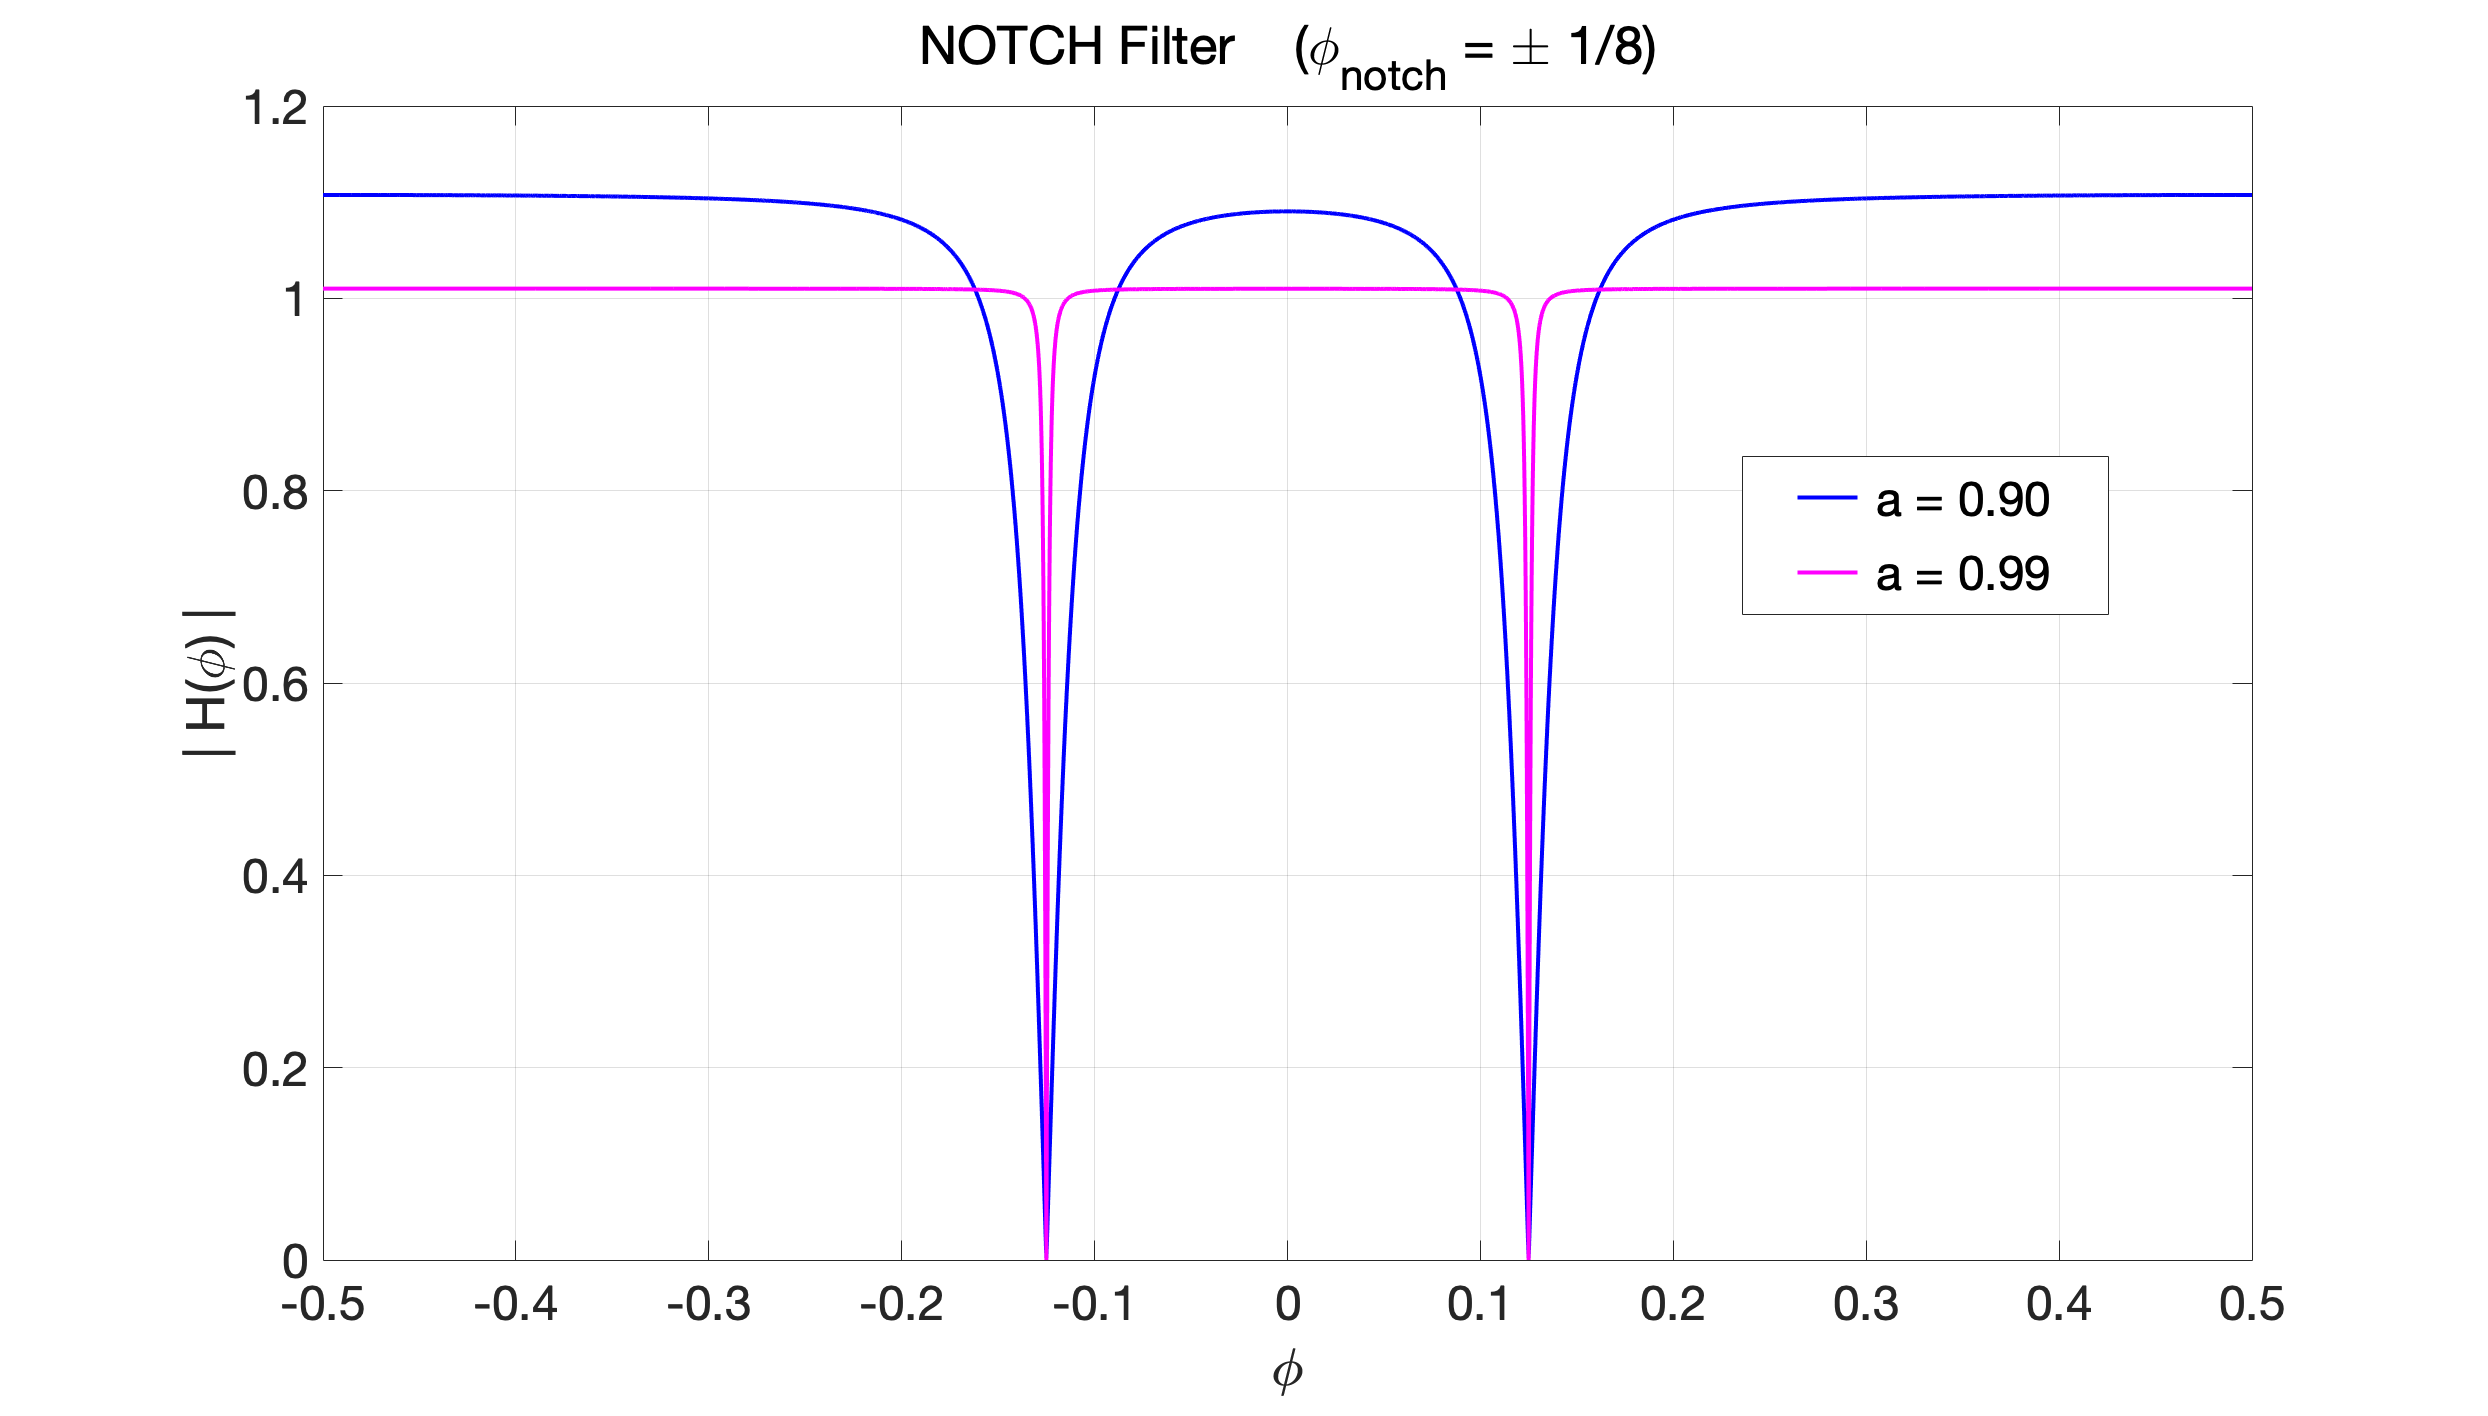
\includegraphics[width=15cm]{src/NotchFilter.png}